\chapter{Realisierung der serverseitigen Implementierung}
\label{cha:server-impl}
In diesem Kapitel wird näher auf die Implementierung des in Kapitel \ref{sec:programmarchitektur} besprochenen Web Services eingegangen. Es enthält eine Übersicht über die genutzten Komponenten und die konkreten Techniken, welche für die Implementierung genutzt wurden. Anschließend wird gesondert auf Sicherheitsaspekte in Verbindung mit \ac{REST}ful-Architekturen eingegangen. Der hier beschriebene Web Service kann über  \textit{\href{http://fit-bachelor.azurewebsites.net/}{http://fit-bachelor.azurewebsites.net/}} erreicht werden. 
\section{Was ist ein Web Service?}
\label{sec:definition-webservice}
Um verteilte Systeme aufzubauen ist es nötig, eine Struktur zu implementieren, mit der Maschinen untereinander kommunizieren können. Diese Aufgabe übernehmen Web Services. Sie stellen innerhalb eines Netzwerkes Schnittstellen bereit, damit Maschinen plattformübergreifend Daten austauschen können. Hierbei wird meistens \ac{HTTP} als Träger-Protokoll genutzt, um eine einfache Interoperabilität zu gewährleisten.\footcite{Definition-Webservice} Die dabei angeforderten Daten werden in der Regel im \textit{\ac{XML}}- oder \textit{\ac{JSON}}-Format übermittelt. 
\subsection{Besonderheiten eines RESTful Web Services}
\label{sec:definition-rest}
Da Web Services in der Regel \ac{HTTP} als Protokoll verwenden, wurde die Idee zur Implementierung eines Web Services erweitert, um die Möglichkeiten des Protokolls besser zu benutzen. Daraus entstand das Programmierparadigma \ac{REST}. Als\ac{REST}-Server bzw. \ac{REST}ful Web Service bezeichnet man einen Web Services, welcher die strikte Nutzung von \ac{HTTP} als Programmierparadigma umsetzt.  Dies meint, dass, wie im Internet üblich, \ac{URI} bzw. \ac{URL} zur eindeutigen Identifikation von Ressource genutzt werden.\footcite[S. 26ff.]{REST-und-HTTP} Diese Ressourcen lassen sich Nachfolgend werden einige Prinzipien von \ac{REST} näher beleuchtet.

\subsubsection*{Adressierbarkeit}
Im Gegensatz zu anderen Web Service-Implementierungen stellen \ac{REST}ful Web Services keine Methoden oder aufrufbare Funktionalitäten zu Verfügung, sondern ausschließlich Ressourcen. Dies hat den Vorteil, dass die Schnittstelle leicht und eindeutig beschrieben werden kann, da ein Aufruf einer \ac{URL} an den \ac{REST}-Service immer eindeutig auf eine Ressource zeigt, ohne, dass Abhängigkeiten oder ein Kontext berücksichtigt werden müssen. \\
In den meisten Fällen, wie auch in den Anwendungsfällen dieser Arbeit, soll der Web Service \textit{\ac{CRUD}}-Funktionalitäten bereitstellen. Damit die Schnittstelle nicht durch unnötig viele unterschiedliche \ac{URL}s überladen wird, sieht der \ac{REST}ful-Ansatz die Verwendung der verschiedenen \ac{HTTP}-Verben vor, um mit den Ressourcen zu Interagieren. Auf die Nutzung von Http-Verben wird im nächsten Abschnitt näher eingegangen. Zur Interaktion mit Ressourcen werden zwei Arten von \ac{URL}s unterschieden, um in Kombination mit \ac{HTTP}-Verben verschiedene Aufgaben zu erfüllen. Zur Veranschaulichung sollen folgende zwei \ac{URL}s dienen:
\begin{itemize}
\item http://myRestService.de/Schedule
\item http://myRestService.de/Schedule/123
\end{itemize}
Es fällt auf, dass die beiden \ac{URL}s sich bis auf das letzte Segment gleichen. Im ersten Fall wird die \ac{URI} als \textit{Collection \ac{URI}} bezeichnet, da hiermit die Gesamtheit aller Trainingspläne angesprochen wird. Im zweiten Fall wird die ID eines Trainingsplans benutzt, um mit einer konkreten Trainingsplan-Ressource zu interagieren. Man spricht dabei von einer \textit{Element \ac{URI}}.\footcite[S. 12ff.]{Building-a-REST-Service} Diese können mit verschiedenen \ac{HTTP}-Verben kombiniert werden.\footcite[S. 26ff.]{REST-und-HTTP}
\subsubsection*{Nutzung von HTTP-Verben}
Um den Rahmen der Arbeit nicht zu übersteigen, wird hier nur auf vier meist verwendeten \ac{HTTP}-Verben beschränkt:\\
Das Verb GET ruft eine Ressource vom Server ab, wobei diese nicht verändert wird. Bei Nutzung einer \textit{Collection \ac{URI}}, werden alle Einträge dieser Entität als Verbundstruktur abgerufen. Jedes Element der Struktur beinhaltet die \textit{Element URI} auf das konkrete Element. Wird GET auf eine \textit{Element URI} aufgerufen, wird das konkrete Objekt aufgerufen. Hierbei antwortet der Server, dem \ac{HTTP}-Standard folgend, mit dem Status-Code \textit{200 (OK)} bei erfolgreicher Suche oder \textit{404 (Not Found)}, wenn keine Ressource gefunden wurde.\\
Das POST-Verb wird zur Erstellung neuer Inhalte verwendet. Bei Nutzung von \textit{Element \ac{URI}s} wird versucht, die ID für das neue Element zu benutzten. In der Regel wird das ID-Management aber auf dem Server implementiert, sodass eine \textit{Collection \ac{URI}} zur Erstellung von Elementen zum Einsatz kommt.\\
Mit dem HTTP-Verb PUT wird eine vorhandene Ressource geändert oder hinzugefügt. Obwohl es \ac{REST}-konform wäre, eine Collection \ac{URI} per PUT aufzurufen, wird dies selten implementiert, da der normale Anwendungsfall darin besteht, dass ein einzelnes Objekt geändert werden soll. Stattdessen wird sich auf \textit{Element \ac{URI}s} beschränkt. Ist eine Ressource mit der übergebenen ID nicht vorhanden, wird je nach Implementierung entweder ein neues Objekt mit der ID erstellt (\textit{Statuscode 201 (Created)}) oder die Verarbeitung verweigert. Der Server gibt dann den Statuscode \textit{400 (Bad Request)} oder \textit{404 (Not Found)}  zurück. \\
Das letzte \ac{HTTP}-Verb, welches an dieser Stelle vorgestellt werden soll, ist DELETE. Wie der Name vermuten lässt, wird damit eine Ressource vom Server entfernt. Wie auch bei PUT wird in der Regel auf eine Implementierung von DELETE als \textit{Collection \ac{URI}} verzichtet, da sonst alle Einträge einer Entität gelöscht werden können. Im Erfolgsfall wird mit dem Statuscode \textit{200 (Ok)} geantwortet und bei Fehlern mit \textit{400 (Bad Request)} oder \textit{404 (Not Found)}.\footcite[S. 26ff.]{REST-und-HTTP}
\subsubsection*{Zustandslosigkeit}
Das zum Datenaustausch genutzte Protokoll \ac{HTTP} ist statuslos. Das bedeutet, dass kein Kontext bei der Kommunikation besteht bzw. jede Kommunikation unabhängig von vor- oder nachherigen Verbindungen ist. Deshalb muss ein \ac{REST}ful Web Service so implementieren werden, dass alle Informationen, welche für die Kommunikation notwendig sind, bei jeder Anfrage mitgesendet werden. Was vordergründig als Nachteil erscheint, ist ein wesentlicher Vorteil. Dadurch, dass jeder Request alle nötigen Informationen mitliefert, ist es nicht nötig, den Kontext der Kommunikation über mehrere Requests auf dem Server zu verwalten. Dadurch kann ein \ac{REST}ful Web Service sehr leicht skaliert werden.\footcite[S. 26ff.]{REST-und-HTTP}
\subsubsection*{Daten sind unabhängig von der Präsentation}
Das \ac{REST}ful-Paradigma besagt, dass Daten losgelöst von einer Darstellung bereitgestellt werden. Darum ist ein \ac{REST}ful Web Service so zu implementieren, dass der Client das gewünschte Datenformat anfragen kann. Bei Nutzung des Protokolls HTTP wird dies in der Regel über die Header-Eigenschaft \textit{accept} realisiert, welche gewünschten Datenformate angibt. Werden dieses nicht vom Server unterstützt, werden die angeforderten Daten in einem Standard-Format zurückgegeben. \footcite[S. 26ff.]{REST-und-HTTP}
\section{Aufbau der Komponenten}
\label{sec:aufbau-Komponenten}
In diesem Abschnitt wird beschrieben, wie der zuvor theoretisch beschriebene \ac{REST}-Ansatz für das Projekt umgesetzt wurde. Der aus der Umsetzung entstandene Server besteht aus zwei Teilen: Der Datenbank und der Web \ac{API}, welche jeweils gesondert vorgestellt werden. \\
Die Web \ac{API} bietet eine Schnittstelle zum Abrufen der Daten mittels \ac{HTTP}. Diese wurde nach dem Design-Pattern \textit{\ac{MVVM}} aufgebaut. Die erzeugten Objekte, welche Tupel einer Datenbank-Relation darstellen, werden aus speziell dafür präparierten Model-Klassen erzeugt. Bevor diese Daten dann über die Web \ac{API} bereitgestellt werden, werden sie vom Model in ein ViewModel übertragen. Hierbei wird, nach dem Grundgedanken des \gls{Seperation-of-Concerns}, klar zwischen den Models für die Datenbank und den ViewModels, welche die Web \ac{API} benutzt, unterschieden.
\subsection{Datenbank}
\label{ssec:aufbau-server-db}
Wie bereits in Kapitel \ref{sec:DB-System} vorgestellt, wurde die Datenbank-Lösung \textit{\ac{MSSQL}} von \textit{Microsoft} zur Datenhaltung gewählt. Dies hat den Vorteil, dass das \textit{\gls{MSEF}}, welches sehr gut für die Nutzung mit einer Web \ac{API} optimiert ist, als \gls{OR-Mapper} genutzt werden kann. Dieser bietet das Design-Pattern \textit{Code First}. Das bedeutet, dass anhand präparierter Model-Klassen die benötigten Relationen in der Datenbank automatisch erzeugt werden. \footcite{entity-framework-code-first}\\
An den folgenden Beispielen wird exemplarisch beschrieben, wie die Model-Klassen aufgebaut wurden und wie sich daraus die Struktur der Datenbank ergibt. Grundlage für die Model-Klassen ist das Interface \textit{IEntity}(Quellcode \ref{lst:IEntity}):
\lstinputlisting[caption=Basisinterface für DB-Repräsentationen, label=lst:IEntity, style=sharpc]{content/listings/IEntity.cs}
Das Interface gewährleistet, dass jede Datenbank-Entität einen eindeutigen Schlüssel besitzt.
Eine konkrete Implementierung für eine Model-Klasse sieht man im \linebreak Quellcode-Beispiel \ref{lst:Schedule}, in der die Trainingspläne implementiert sind:
\lstinputlisting[caption=Modelklasse für Trainingspläne, label=lst:Schedule, style=sharpc]{content/listings/Schedule.cs}
Hierbei zeigt sich gut, was mit einer präparierten Model-Klasse gemeint ist. Über die Annotation \textit{Required} wird definiert, dass die Eigenschaft \textit{Name} zwingend bei Insert- und Update-Operationen gesetzt werden muss. \\
Gleichzeitig sieht man an diesem Beispiel, wie das Entity Framework über Namenskonventionen Verbindungen zwischen Entitäten auflöst. Auf Grund des Aufbaus der Klasse \textit{Schedule} wird eine einwertige Fremdschüssel-Beziehung zu der Model-Klasse \textit{User} erzeugt, da folgende Bedingungen erfüllt sind:
\begin{itemize}
\item Die Klasse \textit{User} besitzt eine Eigenschaft \textit{ID} vom Datentyp \textit{string}
\item Die Klasse \textit{Schedule} besitzt eine Eigenschaft \textit{UserID} vom Datentyp \textit{string}
\end{itemize}
Auch die Erstellung einer mehrwertigen Beziehung lässt sich aus dem Code-Beispiel \ref{lst:Schedule} ablesen: \\
Da es eine Entität gibt, welche \textit{Exercise} heißt und die Model-Klasse \textit{Schedule} eine Verbundstruktur besitzt, welche \textit{Exercises} heißt, wird implizit eine Verbindung zwischen den Relationen in der Datenbank angelegt. \footcite{entity-framework-code-first}
\subsection{Web API}
\label{ssec:aufbau-webapi}
Die Umsetzung der \ac{REST}-Schnittstelle wurde mit Hilfe des \textit{Microsoft}-Frameworks \textit{ASP.NET Web API 2} (kurz \textit{Web \ac{API}-Framework}) realisiert. Dieses ermöglicht es, Controller-Methoden zu erstellen, welche über definierte Routen per \ac{HTTP} aufgerufen werden können. Hierbei wird die Umsetzung im Sinne des \ac{REST}-Paradigmas durch vorhandene Funktionen unterstützt.\footcite[S. 2ff.]{Building-a-REST-Service}\\
Dies wird beispielhaft an der Methode aus  Quellcode-Abbildung \ref{lst:ScheduleController} gezeigt:
\lstinputlisting[caption=POST-Methode zur Erstellung eines Trainingsplans, label=lst:ScheduleController, style=sharpc]{content/listings/SchedulesController.cs}
Im Beispiel fällt auf, dass das \textit{Web \ac{API}-Framework} die Nutzung von Annotationen fördert: Das Routing kann durch die Annotationen \textit{Route} (Zeile \ref{line:SchedulesController_Route}) an der Methode und \textit{RoutePrefix} (Zeile \ref{line:SchedulesController_RoutePrefix}) am gesamten Controller konfiguriert werden. Neben der Konfiguration der Route muss dem Framework noch mitgeteilt werden, welche \ac{HTTP}-Verben in dieser Methode zulässig sind. Das \textit{Web \ac{API}-Framwork} bietet hierfür pro Verb eine eigene Annotation. Im Codebeispiel \ref{lst:ScheduleController} wird über die Annotation \textit{HttpPost} (Zeile \ref{line:SchedulesController_HTTPVerb}) festgelegt, dass nur POST-Requests durch diese Methode verarbeitet werden.\footcite{webApi-AttributeRouting} \\
Das Framework versucht die empfangenen Daten in einem ViewModel-Objekt zu kapseln und anschließend zu validieren. Die dafür genutzten Validatoren werden direkt im View-Model als Annotationen angegeben.\footcite{webApi-Validation} Die Klasse \textit{EntryModel} (Beispiel \ref{lst:EntryModel}) zeigt die Möglichkeit in Zeile \ref{line:EntryModel_Annotation_1} und \ref{line:EntryModel_Annotation_2}. \\ 
\lstinputlisting[caption=Basis-Model-Klasse, label=lst:EntryModel, style=sharpc]{content/listings/EntryModel.cs}
Schlägt die Validierung fehl, werden die Fehler mit dem passenden Statuscode zurückgegeben. Andernfalls werden die Daten per \gls{Factory}-Klasse in ein Model konvertiert und per \gls{Repository}-Klasse in der Datenbank persistiert. Anschließend wird dem ViewModel, im Sinne des \ac{REST}-Gedankens, eine URL zur GET-Methode mit der ID des neu erstellten Objekts übergeben. 
\subsubsection*{Swagger}
\label{sssec:Swagger}
Da die Web \ac{API} zur Entwicklung der Clients benötigt wurde, entstand schnell die Notwendigkeit einer Dokumentation des aktuellen Stands des Web Services. \\
Aus diesem Grund wurde \textit{Swagger} in die Web \ac{API} integriert. \textit{Swagger} ist ein quelloffenes Framework zur Dokumentation von \ac{REST}ful Web \ac{API}s, welche von vielen großen Konzernen genutzt wird\footcite{swagger}. Durch Nutzung des \gls{NuGet}-Packets \textit{Swashbuckle} konnte durch hinzufügen von Kommentaren und Annotationen eine vollständige und übersichtliche Dokumentation erstellt werden\footcite{implementing-Swagger}. Die Abbildung \ref{pic:swagger-UI} zeigt diese. \\
Da das Authorisierungsprotokoll \textit{OAuth} in Version 2 (kurz: \textit{OAuth2} siehe Kapitel \ref{ssec:oauth2}) zum Durchführungszeitpunkt des Projekts noch nicht von \textit{Swagger} unterstützt wird, kann das Ausführen von API-Request aus \textit{Swagger} heraus nur für Methoden durchgeführt werden, für die keine Autorisierung des Nutzers benötigt wird. \\
Die Dokumentation ist unter \textit{\href{http://fit-bachelor.azurewebsites.net/swagger}{http://fit-bachelor.azurewebsites.net/swagger}} aufrufbar. 
\begin{figure}[!h]
\centering
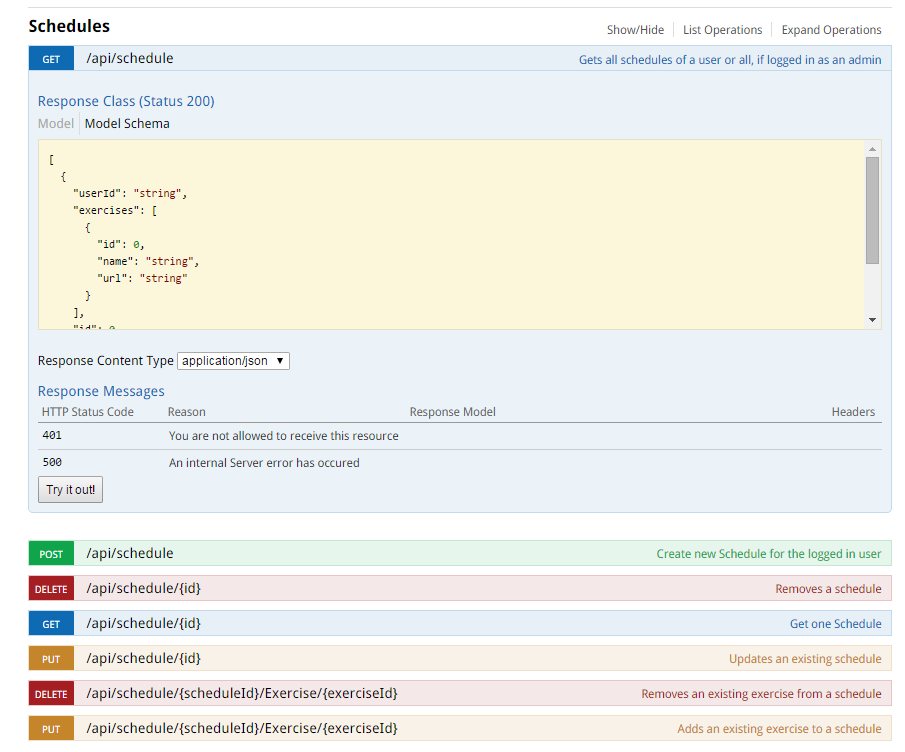
\includegraphics[width=0.8\linewidth]{content/images/Swagger-UI-fIT}
\caption{Swagger UI der Web Api}
\label{pic:swagger-UI}
\end{figure}

\section{Authentifizierung \& Autorisierung}
\label{sec:server-authorisierung}
Wie bereits in Kapitel \ref{sec:rollen-konzept} beschrieben, darf nicht jeder Nutzer auf alle Daten zugreifen. Um dies sicherzustellen, wurde ein Login-Mechanismus implementiert, welcher bekannte Nutzer authentifiziert. Da jedoch nicht alle authentifizierten Nutzer alle bereitgestellten Web \ac{API}-Methoden benutzen, dürfen wurden auf Basis des \textit{\ac{RBAC}} Rollen implementiert, welche den Nutzer zur Nutzung verschiedener Aufrufe autorisieren. Zur Umsetzung dieser Anforderungen wurde das Protokoll \textit{OAuth2} implementiert.\footcite{online:WebApi_Authorize}
\subsection{OAuth2}
\label{ssec:oauth2}
OAuth2 ist ein Protokoll zur Authentifikation und zur Delegation von Zugriffsrollen. Die Struktur von OAuth2 kennt vier Instanzen, welche in diesem Vorgang miteinander kommunizieren. Dazu zählt \textit{Client}, \textit{Resource Owner}, \textit{Authorization Owner} und \textit{Resource Server}.\footcite[S. 286]{book:AngularJs:Steyer2015} 
\begin{figure}[h]
\centering
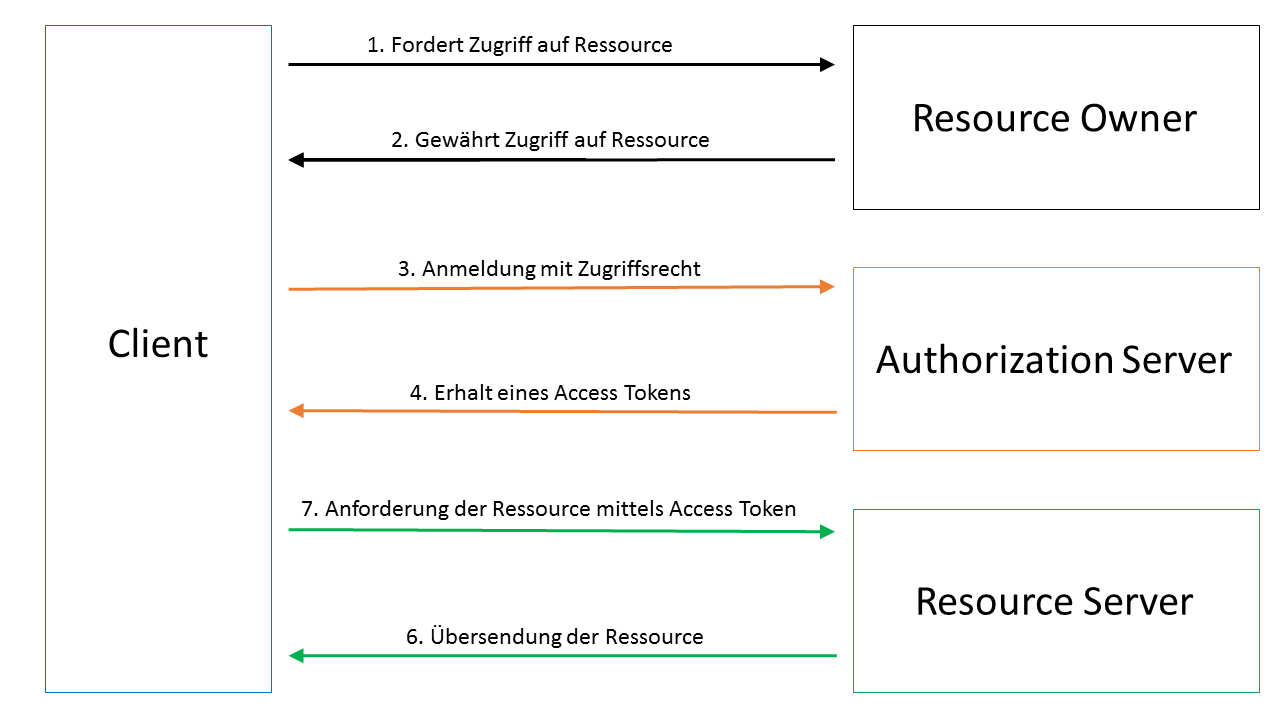
\includegraphics[width=1\linewidth]{content/images/OAuth2}
\caption{Resourcenzugriff durch OAuth2}
\label{pic:OAuth2}
\end{figure}
\subsubsection*{Client}
Der \textit{Client} ist ein Endpunkt, welcher eine Ressource (beispielsweise Trainingspläne) abrufen möchte. In diesem Projekt stellen die Web- und die native App die Clients dar. Diese kommunizieren jeweils mit den anderen Komponenten.
\subsubsection*{Resource Owner}
Der \textit{Resource Owner} ist, wie der Name schon sagt, der Besitzer der geforderten Ressource. Der \textit{Client} erfragt im ersten Schritt beim \textit{Resource Owner} den Zugriff zu einer Ressource.\\
In diesem Projekt registriert sich der Nutzer an der Web \ac{API}. Anschließend kann er unter seinem Account Daten (Trainingspläne und Trainings) anlegen. Diese angelegten Daten sind die geforderten Ressourcen. Da diese vom Nutzer selbst angelegt wurden, erhält er automatisch die Erlaubnis (\textit{Grant}) zur Anfrage am \textit{Authorization Server}\footcite{online:Implemented_OAuth_WebToken}.
\subsubsection*{Authorization Server}
\label{sssec:authorization-server}
Der Nutzer meldet sich nun mit der erhaltenen Erlaubnis am \textit{Authorization Server} an. Dieser hat Kenntnis über alle vorhandenen Nutzer und deren Rollen\footcite{online:Implemented_OAuth_Roles}. Bei erfolgreicher Anmeldung erhält der Nutzer ein kurzlebiges \textit{Access-Token}, dem Typen des Access-Tokens, dessen Ablaufdatum und ein langlebiges \textit{Refresh-Token}. Das Access-Token wird im nächsten Schritt benutzt, um die gewünschte Ressource anzufordern. Das \textit{Refresh-Token} wird benutzt, um ein neues \textit{Access-Token} anzufordern. Die beiden Token-Arten werden nochmal genauer in Abschnitt \ref{ssec:jwt-bearer} besprochen.\footcite[S. 287]{book:AngularJs:Steyer2015} 
\subsubsection*{Resource Server}
Der \textit{Resource Server} enthält die geforderten Ressourcen. Ab diesem Kommunikationsschritt muss das \textit{Access-Token} bei jeder Anfrage mitgesendet werden. Konkret passiert dies, indem der Header der Anfrage um den Schlüssel \textit{authorization} erweitert wird.

Durch diese strikte Trennung dieser Instanzen ist es ohne Weiteres möglich, dass unterschiedliche Systeme die jeweiligen Aufgaben übernehmen. Deshalb hat sich in letzter Zeit etabliert, dass immer häufiger \textit{Single-Sign-On}-Szenarien implementiert werden. Dabei muss ich der Nutzer nur an einer Stelle registrieren (z.B. Bei \textit{Facebook} oder \textit{Twitter}). Will der Nutzer nun auf eine andere Ressource zugreifen, kann der \textit{Ressource-Server} ein \textit{Access-Token} vom \textit{Facebook}-Authorisierungsserver akzeptieren. Dies hat für den Nutzer den Vorteil, dass er sich nicht bei mehreren Seiten registrieren muss, sondern jedes mal Zugriff über den Authorisierungsserver mithilfe seiner \textit{Credentials} erhält. \footcite[S. 294]{book:AngularJs:Steyer2015} 
\subsection{JWT and Bearer Token}
\label{ssec:jwt-bearer}
Sowohl das Access-Token als auch das Refresh-Token sind \ac{JWT}. Das sind codierte und meistens auch signierte Repräsentationen von Daten. Zur genaueren Betrachtung des Aufbaus, wird folgend ein Access-Token näher beschrieben. Es besteht aus 3 Teilen, welche mit einem Punkt voneinander getrennt sind. Die Daten selber sind mithilfe des Kodierungsverfahren \textit{base64} verschlüsselt.\footcite[S. 289]{book:AngularJs:Steyer2015} Die Bestandteile sind:
\begin{itemize}
\item \textbf{Header}\\Hier wird der Typ des Tokens und der Algorithmus, welcher für die Verschlüsselung benutzt wurde, angegeben. 
\item \textbf{Payload} \\Die zu übermittelnden Daten werden als \ac{JSON}-Objekt bereitgestellt. Das Objekt enthält sowohl die Informationen für die Kommunikation, wie beispielsweise den Nutzername und Rollen, als auch Meta-Daten über das Token (z.B. das Ablauf-Datum).
\item \textbf{Signatur}\\Damit gewährleistet ist, dass die Daten unverändert wurden, werden Sie mit einem Client-Secret verschlüsselt. Dies bedeutet aber auch, dass der Server jeden Client kennen muss, welcher sich beim \textit{Authorization Server} anmelden will. \\Da es sich bei diesem Projekt um einen Prototypen handelt, wurde die Implementierung der Client-Verwaltung nicht durchgeführt, da es für den Ablauf nicht zwingend benötigt wird. Der Server lässt alle gültigen Access-Token und alle bekannten Refresh-Tokens zu. Im produktiven Einsatz müsste diese Komponente dringend nachträglich implementiert werden, da sonst eine Sicherheitslücke entsteht.\footcite{online:understanding-jwt}
\end{itemize}
Wie bereits im Abschnitt zum \textit{Authorization Server} (siehe \ref{sssec:authorization-server}) beschrieben, wird für das \textit{Access-Token} eine recht kurze- und für das \textit{Refresh-Token} eine sehr lange Lebenszeit gewählt. Dies hat zwei Vorteile:\\
Das \textit{Access-Token} wird bei Request an den Server mitgesendet. Sollte das Token von Dritten abgefangen werden, können diese nur für kurze Zeit im Namen des Nutzers Aktionen durchführen. Das Abgreifen eines solchen Tokens wird im produktiven Gebrauch durch zusätzliche Sicherheitsmaßnahmen, wie die Nutzung des Protokolls \textit{\ac{HTTPS}} erschwert. \\
Da das \textit{Refresh-Token} ausschließlich zum Erneuern des Access-Tokens benutzt wird, ist die Gefahr, dass es abgefangen wird wesentlich geringer, wodurch die lange Lebensdauer vertretbar ist. \\
Außerdem bleiben durch die kurze Lebensdauer des \textit{Access-Tokens} die Daten immer aktuell. Sollte sich an den Daten des Nutzers etwas ändern (z.B. wird eine Rolle hinzugefügt oder entzogen) wird diese Änderungen beim nächsten Abrufen eines \textit{Access-Tokens} in die Payload codiert\footcite{online:Implemented_OAuth_RefreshToken}. Somit ist immer gewährleistet, das der Nutzer nur die Funktionalität nutzt, für die er auch autorisiert ist. 
\subsection{Zugriff per CORS}
\label{ssec:cors}
Im vorherigen Abschnitt wurden Maßnahmen beschrieben, damit nur autorisierte Nutzer an geschützte Daten herankommen. Mit \textit{\ac{CORS}} wird ein weiterer Mechanismus vorgestellt, welcher den Zugriff auf die Daten per \textit{\ac{AJAX}} beschränkt. \\
Um den Nutzer davor zu schützen, dass eine Webseite im Hintergrund Daten von anderen Quellen nachlädt, ist in jedem Browser eine \textit{Same-Origin-Policy} implementiert. Diese besagt, dass nur Daten aus der gleichen Domäne, aus der der \textit{\ac{AJAX}}-Aufruf abgesetzt wurde, abgerufen werden dürfen. \\
Da es trotzdem häufig nötig ist, auf fremden Domänen zuzugreifen, wurden schnell Hilfskonstrukte wie das Vorgehensmodell \textit{\gls{JSONP}} eingeführt. Da diese jedoch von vielen Entwicklern als nicht elegant empfunden wurden\footcite[S. 102]{book:AngularJs:Steyer2015}, wurde mit \ac{CORS} ein standardisierter Weg entwickelt, um Daten von fremden Domänen abzurufen. \\
Hierbei wird beim Server eine Liste an gültigen Domänen für eine domänenübergreifende Anfrage hinterlegt. Soll nun vom Browser eine Anfrage an den Server gesendet werden, wird über das \ac{HTTP} Verb unterschieden, ob durch diese Anfrage eine Server-Datum verändert wird. Dies geschieht bei PUT, DELETE und POST, wobei letzteres eine Ausnahme bildet. Werden per POST Daten in einem Format übermittelt, welches beim Absenden eines Formulars genutzt wird (z.B. \textit{application/x-www-form-urlencoded}), wird die Anfrage wie ein nicht-ändernder Aufruf behandelt. \\
Wenn nun eine Datenänderung im Sinne von \ac{CORS} durch den Aufruf angestoßen wurde oder wenn der Aufruf zusätzliche Schlüssel im Header enthält, wird vor der Ausführung ein \textit{Preflight} gesendet. Dies ist eine gls{OPTIONS}-Anfrage, welche genutzt wird, um die Durchführung der bevorstehenden Anfrage zu validieren.
Enthält die Antwort im Header nicht den Schlüssel \textit{Access-Control-Allow-Origin} mit der aufrufenden Domäne, wird vom Browser ein Fehler erzeugt. Andernfalls wird die Abfrage an den Server gesendet\footcite[S. 102]{book:AngularJs:Steyer2015}. Dadurch ist gewährleistet, dass nur berechtigte Clients anfragen an den Server senden. Es wurde auf weitere Implementierung von \gls{Polyfills} verzichtet, da \ac{CORS} bereits in allen modernen Browsern genutzt werden kann\footcite{online:can-i-use:cors}.
\section{Testen der Funktionalität}
\label{sec:server-tests}
Die erwartete Funktionsweise des Servers ist Grundvoraussetzung für die Umsetzung der Clients. Um diese zu bewerkstelligen wurde die \textit{ManagementApi} entwickelt. Dies ist eine portable \ac{DLL}, welche alle Anfragen an den Server in Methoden kapselt. Hierbei wurde bei der Erstellung der \ac{DLL} darauf geachtet, dass sie sowohl in klassischen Testprojekten als auch zur Umsetzung der nativen App genutzt werden kann. Darüber hinaus war ein Design-Ziel, dass alle Methode auch asynchron aufrufbar sind, damit Nutzer der \ac{DLL} in der Erstellung Ihres Programmablaufes größere Flexibilität besitzen. \\
Die erzeugten Methoden wurden iterativ entwickelt und direkt getestet. Hierbei wurden zur Verifikation der Funktionalität ausschließlich Positivtests erstellt. So war sichergestellt, dass jede Methode der \textit{ManagementApi} die gewünschten Aktionen auf dem Web Service durchführt. \\
Der nachfolgende Codeausschnitt zeigt beispielhaft die Entwicklung eines Testfalls:
\lstinputlisting[caption=Implementierung des Tests 'Nutzer kann eigene Daten anpassen', label=lst:ClientTests.Users, style=sharpc]{content/listings/ClientTests.Users.cs}
Dadurch, dass die Klassen \textit{ManagementService} und \textit{ManagementSession} das Interface \textit{IDisposable} implementieren, kann für jeden Test unabhängig eine neue Session erstellt werden, in der der Test läuft. Ist der \textit{using}-Block vollständig durchlaufen, wird die \textit{Dispose}-Methode aufgerufen, welche die verwendeten Ressourcen wieder freigibt (siehe Zeile \ref{line:ClientTests:Disposable}f.). 